\expandafter\ifx\csname ifdraft\endcsname\relax
\documentclass[11pt]{jsreport}
\usepackage{mypackage}
\begin{document}
\fi

\chapter{本手法による不具合分析の実践と評価}

\section{概要}
不具合分析の具体的な流れをみるために,いくつかの事例を取り上げて実践した結果を示す.
以下では,まず実際に故障箇所特定が行えた事例を取り上げる.
その結果に関して,コマンドを選択する際に優先する指標を変えることによって検証プロセスが異なること
を述べ,評価指標に関する考察を行う.
次に,故障箇所の特定を上手くできなかった事例を取り上げ,
そこから得られた知見に関して述べる.
%ここら辺もう少し見るところがある気がする.
%こんなことゆってないぞ
最後に,本手法によって扱うことのできる故障の種類に関する限界を述べ,発展させるために必要な
方針に関して議論を行う.

\section{実践例}
%もう少しsectionわけの名前を考える.
\subsection{故障箇所の特定ができた例(ヒータの接触不良)}
まず,以下の図\ref{fig:fault_mode1}のような故障を考え,
不具合分析を行っていく.\\
%図の配置を考える.
\begin{figure}[H]
   \centering
      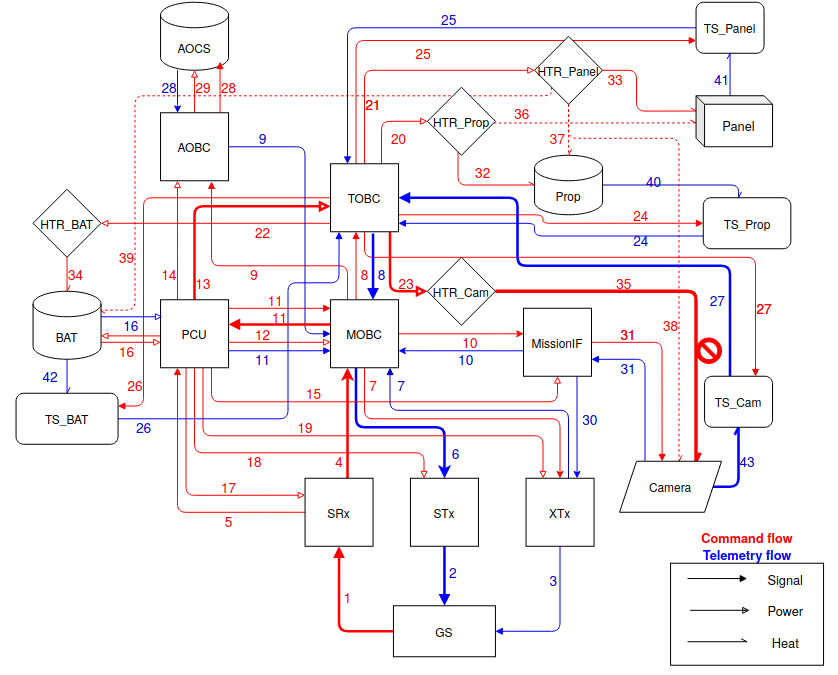
\includegraphics[height=13.0cm]{figure/fault_mode1.png}
      \caption{故障箇所:リンク32(推進系ヒータ−推進系間)の時の故障候補}
      \label{fig:fault_mode1}
\end{figure}

%問題設定の与え方として,各コンポーネントの状態はどのようになっているかを示したほうが良くないか?
%Methodologyの中で言及できているのか要確認
図\ref{fig:fault_mode1}に示すような
推進系ヒータ‐推進系間でのヒータ接触不良が発生している場合を考える.
この時,異常検知の際の不具合事象としては,
\begin{itemize}
   \item 推進系ヒータONコマンド(ID:14)を送信したのに,推進系温度(ID:17)が上昇しない
\end{itemize}
という事象である.\\
%つまりは正常モデルを元に考えているからこうなる
ここで,本手法では前章で述べたように衛星内部コンポーネントの初期状態として,
送信したコマンドによってもたらされる状態変化が起こっているものとして与えている.
そのため,不具合事象の際に送っているコマンド「推進系ヒータON」によって,
推進系ヒータは電源ON状態であると仮定し,以下の検証用コマンドの探索を行っている
ことを述べておく.
%これ実は別にどっちの状態にしてても,検証はできるんやけどな..
%ほんまは不具合検知コマンドとテレメトリのペアを除外する必要はないんかもな...

以下に,この事象に本手法を適用した例を示す.
まず,図\ref{fig:tel_phase}に
故障候補の決定及び,テレメトリ情報を用いた確認の段階を示す.
故障候補の決定では,不具合事象を検知するきっかけとなったコマンドとテレメトリが形成する
経路を探索し,targetTEL,targetCOMとして提示している.\\
その後,時間変化するテレメトリ情報を用いて確認できる故障候補を提示し,
返ってくるテレメトリが正常(OK)か否(NG)かを入力させることで,切り分けを行っている.
今回の例ではMOBC及びTOBCは正常に動作しているはずなので,MOBCカウンタ及びTOBCカウンタは正常(OK)
と入力し,それを元に状態の更新を行っている.
\begin{figure}[H]
   \centering
      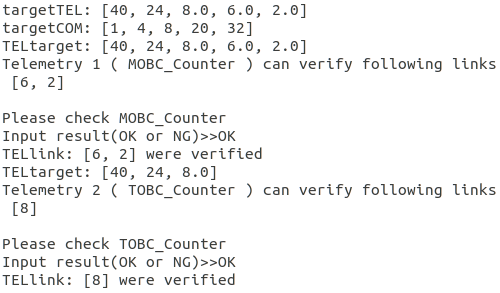
\includegraphics[height=5.0cm]{figure/COM14_TEL17_TEL_phase.png}
      \caption{テレメトリによる確認}
      \label{fig:tel_phase}
\end{figure}
次に,図\ref{fig:ini_COM_phase}に示すのが,不具合発生時に送信していたコマンド情報から
考えられるテレメトリの変化を用いて故障候補の確認を行う段階である.
今回は,初期コマンドとしては異常検知の際に送ったコマンド(推進系ヒータON)のみ
を考えている.
確認可能性の高い経路を形成するテレメトリから順に表示され,人間に確認をさせているのが分かる.
ここでの確認テレメトリに関しても,今回の例では正常であるため,そのように入力し状態の更新
を行っている.
%もう少し説明が必要そう
\begin{figure}[H]
   \centering
      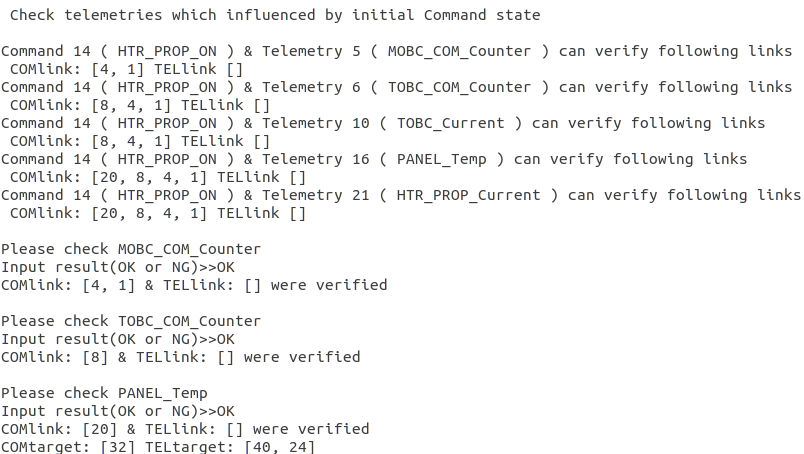
\includegraphics[height=7.0cm]{figure/COM14_TEL17_iniCOM_phase.png}
      \caption{初期コマンドを用いた確認}
      \label{fig:ini_COM_phase}
\end{figure}

最後に,以下の図\ref{fig:COM_candidate}に示すのが,上記の流れを経て残った
故障候補を確認できるコマンドを探索し,指標と共に提示した結果である.
残った故障候補は,
\begin{itemize}
   \item コマンドリンク32:推進系ヒータ‐推進系間
   \item テレメトリリンク40:推進系‐推進系温度計間
   \item テレメトリリンク24:推進系温度計‐TOBC間   
\end{itemize}
である.
この時,探索結果として表示されたのはコマンド13(パネルヒータON)と18(推進系ヒータOFF)
であり,これらのコマンドに関する指標が図\ref{fig:COM_candidate}のように示されている.\\
図中においてPm(C)が「平均確認可能性」,E(C)が「確認可能リンク数」,
N(C)が「検証コマンド総数」を表している.
またコマンドの衛星生存性への副作用を示す指標に関しては,
Remain Powerが「コマンド送信前のバッテリ残量」,Power Consume
「コマンド送信による消費電力」,
Impacted TEL numが「コマンドによって影響を受けるテレメトリの数」,
Attitudeが「姿勢変化を起こすか否か」を示している.
Attitudeに関しては,姿勢変化を起こす場合は"Change",起こさない場合は"Keep"と表示するようにしている.

\begin{figure}[H]
   \centering
      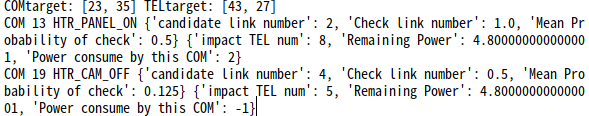
\includegraphics[width=15.0cm]{figure/COM_candidate.png}
      \caption{コマンドの選択肢表示及び検証過程}
      \label{fig:COM_candidate}
\end{figure}
以下の図\ref{fig:COM_process_HTR_fault}に,探索されたコマンドに関して各コマンドを選択し
検証を行ったプロセスを示す.
どちらのコマンドから開始しても最終的に,今回想定した故障箇所である「推進系ヒータ−推進系間(リンクID:32)」
が故障箇所であると特定された.

\begin{figure}[H]
   \centering
      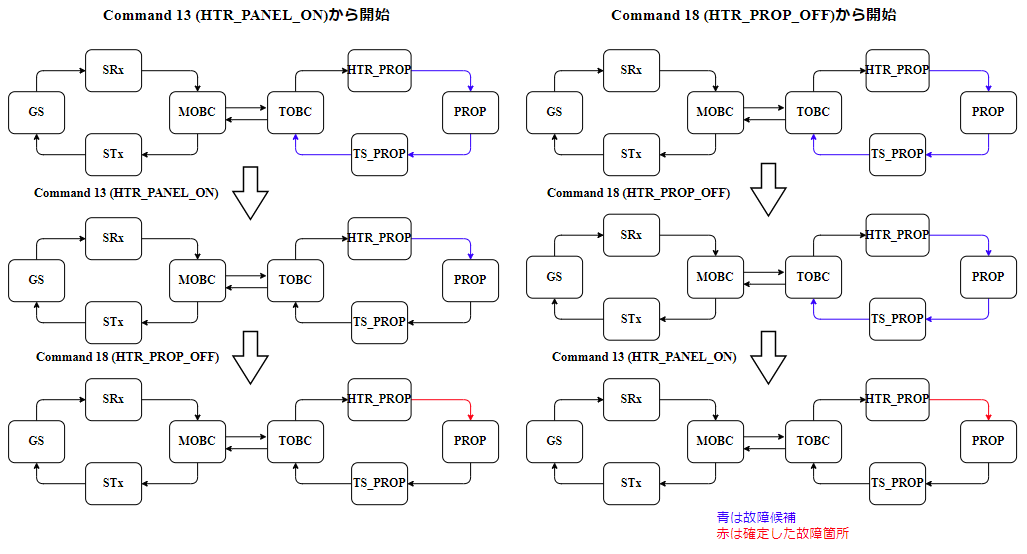
\includegraphics[height=8.0cm]{figure/COM_process_HTR_PROP_fault.png}
      \caption{ヒータ接触不良時の各検証プロセスの流れ}
      \label{fig:COM_process_HTR_fault}
\end{figure}
%結果に関して何か..


\subsection{評価指標に関する考察}
%ここの文言も微妙
上で示した例(ヒータ接触不良)に関して,コマンドを選択する際に優先する評価指標によって
図\ref{fig:COM_process_HTR_fault}のように検証プロセスの違いが生じた.
この結果の違いに基づき,提示された評価指標が持つ意味を考察する.

図\ref{fig:COM_candidate}にあるように提示された2つのコマンドを比較すると,
「平均確認可能性」はパネルヒータONコマンド(13:HTR\_PANEL\_ON)が高く,
「検証コマンド総数」は推進系ヒータOFFコマンド(18:HTR\_PROP\_OFF)が小さくなっている.
パネルヒータONコマンドから検証を開始した場合,初めに
「推進系−推進系温度計間(テレメトリリンク40)」,「推進系温度計−TOBC間(テレメトリリンク24)」
の正常が確認できており,
1つのコマンドによる確認で故障候補が1つのリンクにまで絞り込めている.
最終的に,推進系ヒータOFFコマンドを送信した際に%何のテレメトリで??
推進系温度の変化が見られなかったことから「推進系−推進系温度計間(テレメトリリンク32)」
の異常が確認でき,故障箇所を特定している.\\
一方で,推進系ヒータOFFコマンドから検証を開始した場合,
1つ目の検証では推進系温度に変化が見られず,状態変化を確認できないため,
故障候補の切り分けをすることができない.一方で,故障候補の中に
確実に故障箇所が存在することを確かめることができる.
次に,2つ目のコマンド「パネルヒータON」で推進系温度の上昇を見ることができるため,
先程のプロセスと同様の切り分けができ,故障箇所の特定ができている.

運用時,通信が不安定であり不具合分析に使える時間が明確でない時には
一度のコマンドで多くの確認ができることが望ましい.
そのため,図\ref{fig:COM_candidate}において「パネルヒータON」コマンドから送信する
検証プロセスが良いと言える.
これを元に考えると,
平均確認可能性が高いコマンドから送ると,一回のコマンドで多くの絞り込みが行える可能性が高いと言える.
より厳しい時間制約の際には,最後まで検証作業を行うことができるという保証はない.
そのため,平均確認可能性が高いコマンドを優先的に選択して各コマンドによって得られる切り分けの効果を
大きくすることが望ましい.

一方で検証コマンド総数が小さなコマンドを優先的に選択した場合,
少ないコマンド数で絞り込みを行える可能性があるが,
この指標はあくまで,故障箇所を特定するまで検証を行うことを前提としてコマンドの数を計算している.
そのため,故障状態によっては
見積もられた数以上のコマンドを送信する必要があり,時間制約が厳しいときには十分に
絞り込みを行えないまま検証作業を終えることになる.
このことを踏まえると,検証コマンド総数は不具合分析を最後まで行うことができる保証がある時に,
優先的に考えることで,全体で打つコマンドの数を少なくできる可能性があると言える.

%複数故障を考えた場合,指標の選択基準によって
%探索プロセスが変化する.

%別で特定できなかった事例を取り上げて設計へのフィードバック.
%評価指標の優先順位を考えることでどのように検証結果が変化するのかを考察する.
\subsection{温度計故障に関する検証}%???
次に,以下の図\ref{fig:fault_mode2}に示すような
温度計故障(断線)を考え検証を行った例に関して述べる.
この時,異常検知の際の不具合事象としては,上の事例と同じく
\begin{itemize}
   \item 推進系ヒータONコマンド(ID:14)を送信したのに,推進系温度(ID:17)が上昇しない
\end{itemize}
という事象である.
テレメトリの確認や,初期コマンド状態からの確認情報の提示の流れは先ほどの例と
同様となる.
\begin{figure}[H]
   \centering
      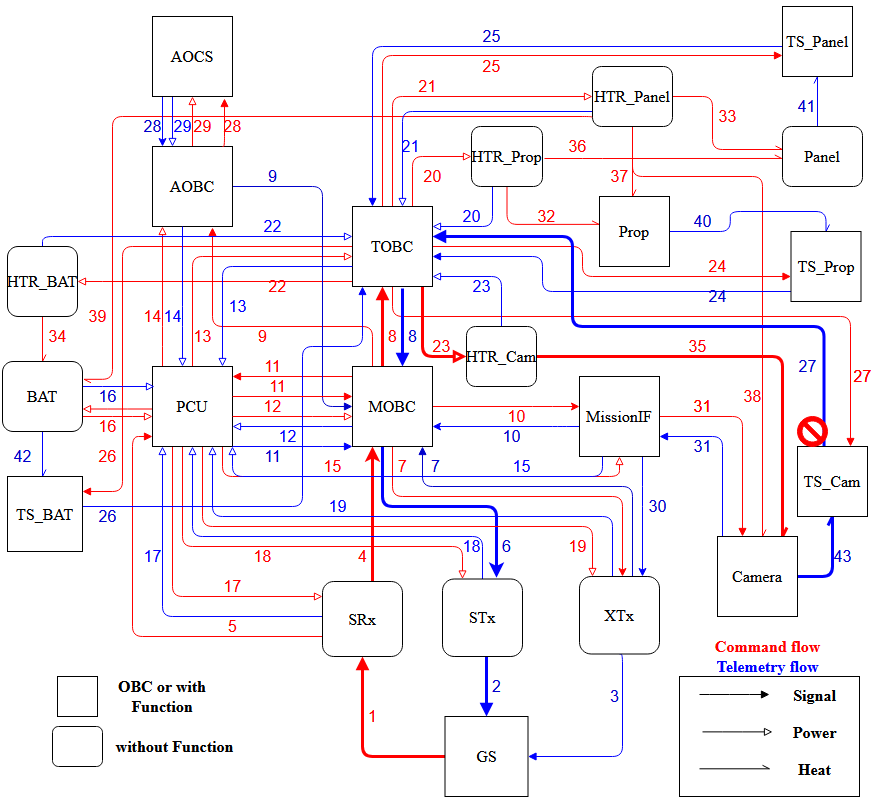
\includegraphics[height=13.0cm]{figure/fault_mode2.png}
      \caption{故障箇所:リンク24(推進系温度計-TOBC間)の時の故障候補}
      \label{fig:fault_mode2}
\end{figure}
この時,システムによって洗い出された検証用のコマンドは上の例(図\ref{fig:COM_candidate})
のものと同じであり,指標から判断するとコマンド13の方が切り分けられるリンクの数は大きい一方で
全体のコマンド数の見積もりでは,コマンド18の方が少ないコマンド数であるという結果になっている.
コマンド13及び18を初めに選択した結果はそれぞれ以下の図\ref{fig:COM13_start},\ref{fig:COM18_start}
のようになった.
今回の不具合は温度計の断線であるため,パネルヒータによる推進系温度の変化も
推進系ヒータによる推進系温度変化も見ることはできないため,どちらも入力は異常(NG)を与えている.
最終的な結果は,どちらの過程を経ても同じになっており,
一つのリンクにまで故障箇所の特定を行うことができなかった.
このことから,この衛星モデルが今回扱った故障「(推進系)温度計故障」が発生した際に故障特定を行える設計
になっていないことが分かる.
このように,本手法は単に故障箇所の特定を支援するだけでなく,設計の不備を洗い出すことにも
利用できる.
%ここからやる!!!

\begin{figure}[H]
   \centering
      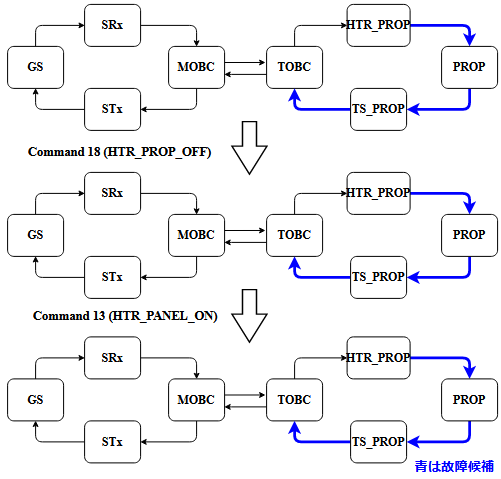
\includegraphics[height=8.0cm]{figure/COM_process_TS_fault.png}
      \caption{温度計故障時の検証プロセスの流れ}
      \label{fig:COM_process_TS_fault}
\end{figure}

本研究で構築したシステム上では故障箇所の特定までを行うことができなかったが,不具合分析の過程で得た情報
を用いて人間側で故障箇所の類推をすることは可能である.
今回の事例では,コマンドリンク20が正常であることは「パネル温度」によって確認できており,
パネル温度の上昇を確認することでヒータの正常が動作していることも確認できるため,推進系ヒータの故障ではない
ことが分かる.また,「パネルヒータON」によって推進系温度の変化を見ることができなかったことから,
テレメトリリンク:40,24が異常であることも類推できる.このように,本システムに従って検証を行うことによって,
故障箇所の推論するために必要な情報が取得可能であることがわかる.

実ミッションでは,設計段階においてFMEA(Failure Mode and Effect Analysis)などを用いて,
衛星システムに起こりうる故障モードを列挙し,それらの故障モードによる影響や,
発見のしやすさなどをもとに設計へのフィードバックを行う.よって,FMEA上で洗い出された
故障モードに対して本手法を適用することによって,それぞれの故障モードが発見可能な設計になっているか
を確認することができる.


\begin{comment}
まず,MOBCとTOBCからテレメトリは全て降ろされているものと仮定する.
また,故障は「推進系ヒータの接着不良」であるとする.
その時,テレメトリを通して確認できるのは
\begin{itemize}
   \item 「推進系ヒータON」コマンドを送ったのに,「推進系温度」テレメトリが変化しない.
\end{itemize}
という事象である.
よって不具合検知は,この事象によって行われる.

\subsection{不具合分析の例}
この不具合において,「推進系ヒータON」コマンドを送信して推進系ヒータに熱が伝わるまでの経路
と,推進系温度計が温度を読み取り「推進系温度」テレメトリとして地上局に伝わるまでの
経路の中に故障箇所があると考えることができる.
この経路を以下の図\ref{fig:simple_sat_fault}に太矢印で示している.
%これにリンクID入れたら見やすいかも
\begin{figure}[H]
   \centering
      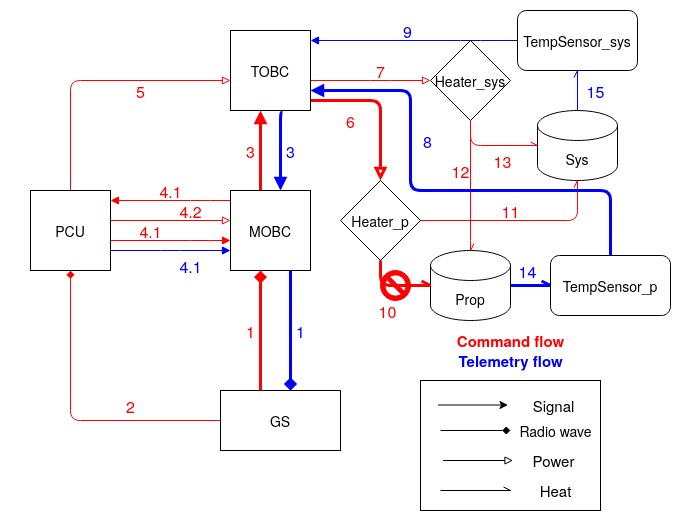
\includegraphics[height=9.0cm]{figure/simple_sat_fault.png}
      \caption{故障箇所と不具合検知に関連するコマンドとテレメトリの経路}
      \label{fig:simple_sat_fault}
\end{figure}
また,この経路内にあるコンポーネントに電源が入っているかどうかを確認するためには,
そのコンポーネントに電源を供給するための経路が正常に作動しているかどうかを確認する
必要がある.そこで
\begin{itemize}
   \item PCU$\rightarrow$MOBC(リンクID:4.2),PCU$\rightarrow$TOBC(リンクID:5)
\end{itemize}
も検証を行う対象として考える.
以上より,検証すべき経路は下記のようになる.
\begin{itemize}
   \item コンポーネント:GS,MOBC,TOBC,Heater\_p,Prop,TempSensor\_p
   \item コマンドリンク:GS-MOBC(1),MOBC-TOBC(3),MOBC-PCU(4.2),
   PCU-TOBC(5),\\TOBC-Heater\_p(6),Heater\_p-Prop(10)
   \item テレメトリリンク:GS-MOBC(1),MOBC-TOBC(3),TOBC-TempSensor\_p(8),
   TempSensor\_p-Prop(14)
\end{itemize}
以下,提案手法によるアルゴリズムによって不具合分析を行っていく.\\
%この章長くて読みにくい
まず,問題設定よりMOBC及びTOBCのテレメトリは全てダウンリンクされている状態に
あるので,
\begin{itemize}
   \item テレメトリリンク:TOBC$\rightarrow$MOBC(3),MOBC$\rightarrow$GS(1)
   \item コマンドリンク:PCU$\rightarrow$MOBC(4.2),PCU$\rightarrow$TOBC(5)
\end{itemize}
は問題ないことが確認できるため,故障可能性はなくなる.
問題設定ではあるが,実際に「MOBC及びTOBCのテレメトリが全てダウンリンクされている」
ことを確認するためには,「MOBCカウンター」
「TOBCカウンター」を確認することが必要である.\\
また不具合発生時,推進系ヒータが正常に作動しており,
システム温度計からテレメトリを下ろす経路に問題がなければ,
「システム温度」が上昇しているはずである.
よって,テレメトリの確認によって検証できる経路として,
コマンドリンク「TOBC-Heater\_p(6)」がある.
以上より,不具合発生時から状態変化させずに確認すべき事項として以下
が挙げられる.

\begin{table}[H]
   \centering
   \caption{コマンドなしでの確認事項} 
   \label{tab:check_list1}
\end{table}
\vspace{-2zh}
\begin{figure}[H]
   \centering
      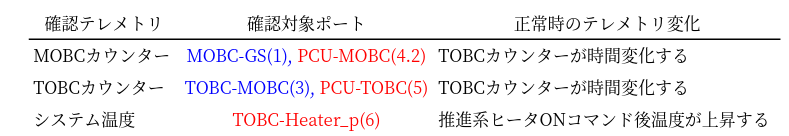
\includegraphics[height=2.5cm]{figure/check_list_tel.png}
\end{figure}
衛星の状態を変化させること無く,テレメトリを確認するだけで
検証できる箇所はこれ以上存在しないので,次にコマンドによる検証を行う.

まず,コマンドパスとしてGSに近い箇所から順に確認を行う必要がある.
MOBCへのコマンドが通っているかを確認するためには,「MOBCコマンドカウンターアップ」
コマンドを送って,「MOBCコマンドカウンター」が変化していることを確認できれば良い.
同様に考えると,以下の様に確認事項を洗い出すことができる.
\begin{table}[H]
   \centering
   \caption{コマンド送信による確認事項} 
   \label{tab:check_list2}
\end{table}
\vspace{-2zh}
\begin{figure}[H]
   \centering
      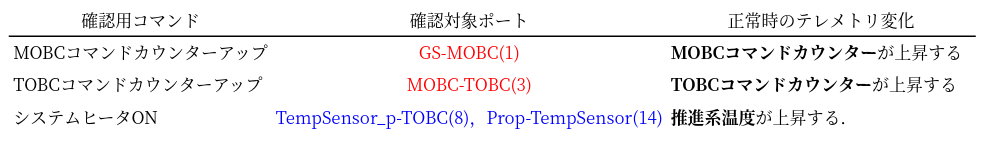
\includegraphics[height=2.6cm]{figure/check_list.png}
\end{figure}
以上の項目を確認した際,今回想定した故障モード(推進系ヒータの接着不良)
では期待されるテレメトリデータの変化が起こるので,
Table \ref{tab:check_list2}の確認対象パスの中にある故障可能性箇所は
棄却され,
故障可能性リンクとして残るのは
\begin{itemize}
   \item コマンドリンク:Heater\_p-Prop(10)
\end{itemize}
となる.

%上のコマンドを送っても大丈夫なのかという議論はどうするのか?もしシステム温度が高いのに,その方法でたしかめてもいいものなのか?

この経路上で考えうる故障モードと照らし合わせると,
この切り分けによって残る故障モードは
\begin{itemize}
   \item 推進系ヒータの故障
   \item 推進系ヒータの接着不良
\end{itemize}
となる.
この時,
「システム温度」の上昇によって「推進系ヒータの故障」の可能性は
棄却できるため,最終的に「推進系ヒータの接着不良」
が残り,
実際の故障を棄却すること無く,絞り込みができていると言える.\\
\end{comment}




\expandafter\ifx\csname ifdraft\endcsname\relax
  \end{document}
\fi